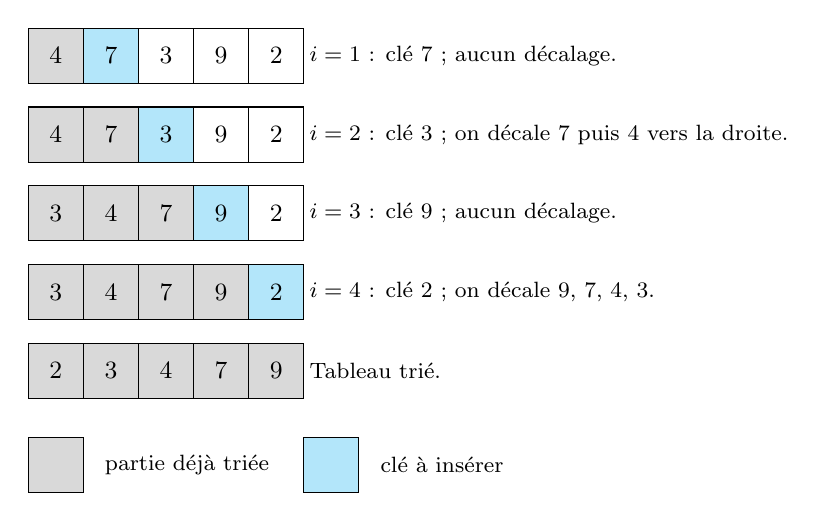
\begin{tikzpicture}[x=1cm,y=1cm,c/.style={draw,minimum size=0.7cm,inner sep=0pt,font=\small},
 mn/.style={fill=orange!45},ok/.style={fill=gray!30},cl/.style={fill=cyan!30},ix/.style={thick,draw=black,line width=1.2pt},hors/.style={text=gray,draw=gray!60},lab/.style={anchor=west,font=\footnotesize,align=left}]
\node[c,ok] at (0.00,0.00) {4};
\node[c,cl] at (0.70,0.00) {7};
\node[c,] at (1.40,0.00) {3};
\node[c,] at (2.10,0.00) {9};
\node[c,] at (2.80,0.00) {2};
\node[lab] at (3.1,0.00) {$i=1$ : clé $7$ ; aucun décalage.};
\node[c,ok] at (0.00,-1.00) {4};
\node[c,ok] at (0.70,-1.00) {7};
\node[c,cl] at (1.40,-1.00) {3};
\node[c,] at (2.10,-1.00) {9};
\node[c,] at (2.80,-1.00) {2};
\node[lab] at (3.1,-1.00) {$i=2$ : clé $3$ ; on décale $7$ puis $4$ vers la droite.};
\node[c,ok] at (0.00,-2.00) {3};
\node[c,ok] at (0.70,-2.00) {4};
\node[c,ok] at (1.40,-2.00) {7};
\node[c,cl] at (2.10,-2.00) {9};
\node[c,] at (2.80,-2.00) {2};
\node[lab] at (3.1,-2.00) {$i=3$ : clé $9$ ; aucun décalage.};
\node[c,ok] at (0.00,-3.00) {3};
\node[c,ok] at (0.70,-3.00) {4};
\node[c,ok] at (1.40,-3.00) {7};
\node[c,ok] at (2.10,-3.00) {9};
\node[c,cl] at (2.80,-3.00) {2};
\node[lab] at (3.1,-3.00) {$i=4$ : clé $2$ ; on décale $9$, $7$, $4$, $3$.};
\node[c,ok] at (0.00,-4.00) {2};
\node[c,ok] at (0.70,-4.00) {3};
\node[c,ok] at (1.40,-4.00) {4};
\node[c,ok] at (2.10,-4.00) {7};
\node[c,ok] at (2.80,-4.00) {9};
\node[lab] at (3.1,-4.00) {Tableau trié.};
\node[c,ok] at (0,-5.2){};\node[lab] at (0.5,-5.2){partie déjà triée};\node[c,cl] at (3.5,-5.2){};\node[lab] at (4.0,-5.2){clé à insérer};
\end{tikzpicture}